\def\leftcircle{(-1,0) circle (2 cm)}
\def\rightcircle{(1,0) circle (2 cm)}
\begin{figure}[H]
  \centering
  \label{tikzpic:set_sym_minus}
   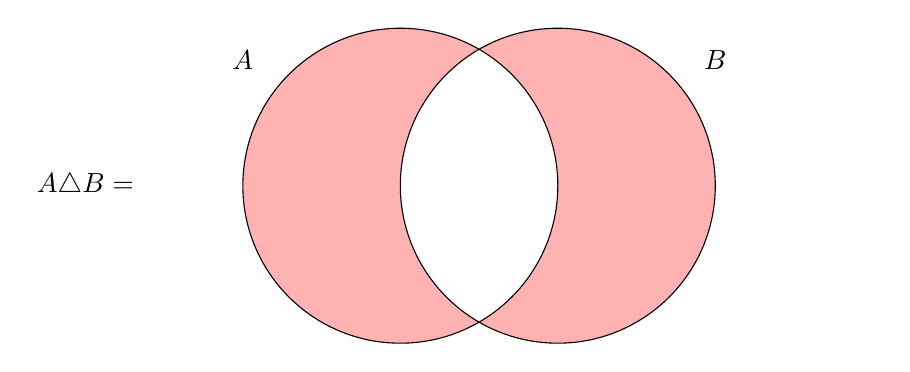
\begin{tikzpicture}
    \begin{scope}
      \clip \rightcircle (-3,-2) rectangle (3,2);;
      \fill[red!30] \leftcircle;
    \end{scope}
    \begin{scope}
      \clip \leftcircle (-3,-2) rectangle (3,2);;
      \fill[red!30] \rightcircle;
    \end{scope}
            
    \draw \leftcircle;
    \draw \rightcircle;
    \draw (-3,1.6) node {$A$};
    \draw (3,1.6) node {$B$};
    \draw (-5,0) node {$A \triangle B = $};
    \draw (5,0) node {\text{     }};
  \end{tikzpicture} 
  \caption{Симметричная разность}
\end{figure}

